\section{VPN Setup}
We can define the \textbf{road warriors}, in our case, as a set of three users - \textit{Becca, Huck and Jim} - which we want to be able to authenticate and then connect to the internal subnetworks in the \textbf{ACME Co.} target network from the \textbf{WAN} interface on the \textbf{Main router} via a \textbf{Virtual Private Network}.\\
To this end, in order to setup a \textbf{VPN} on the \textbf{Main router}, we exploit the \textbf{OPNSense} administration panel and then navigate to \textbf{VPN $->$ OpenVPN $->$ Servers}, where we can \textbf{add a new server} to which the \textbf{road warriors} will refer to authenticate and configure their \textbf{VPN}. \textbf{Figure 1, 2, 3} show the server we created and all the parameters - protocol, port, cryptographic and tunnel settings - that we chose to adopt.\\
\begin{figure}[!htb]
\centering
\begin{minipage}{.33\textwidth}
  \centering
  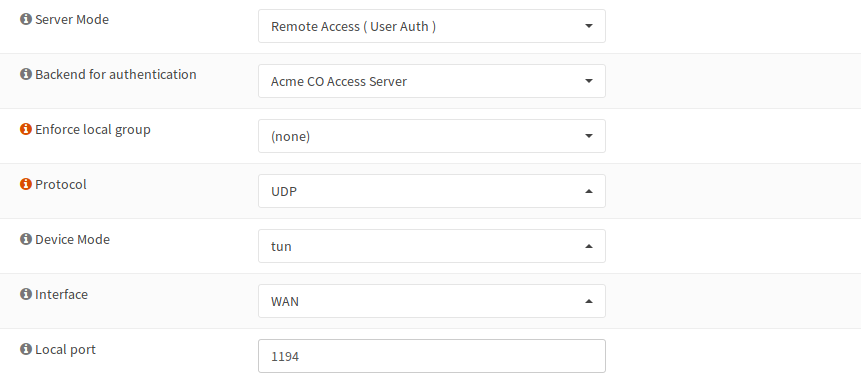
\includegraphics[width=1\textwidth]{vpnserver1.png}
  \caption[a]{VPN Server's general settings with protocol and port.}\label{fig:1}
\end{minipage}%
\begin{minipage}{.33\textwidth}
  \centering
  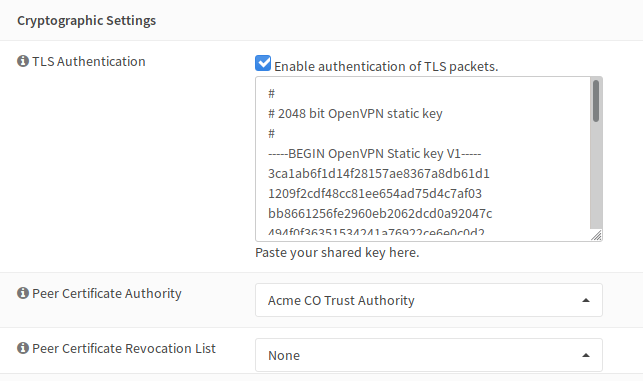
\includegraphics[width=1\textwidth]{vpnserver2.png}
  \caption[a]{VPN Server's crypto settings (1).}\label{fig:2}
\end{minipage}
\begin{minipage}{.33\textwidth}
  \centering
  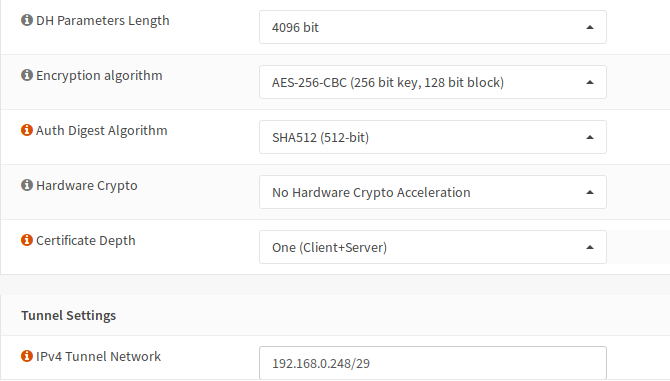
\includegraphics[width=1\textwidth]{vpnserver3.png}
  \caption[a]{VPN Server's crypto settings (2) and IP tunneling address.}\label{fig:3}
\end{minipage}
\end{figure}

Server has been assigned to a \textbf{Server Certificate} signed by the authority - the server itself - which can be given to the clients to prove the server's identity, so to perform server-to-client authentication.\\
Also, under \textbf{System $->$ Servers} we setup a new \textit{Acme CO Access Server} which will be exploited to actually access the \textbf{VPN Server}, exploiting an access strategy based on a \textit{Local Database $+$ Timebased One Time Password}, with the  \textbf{OTP} being provided by \textit{Google Authenticator} and thus having length 6. Before actually implementing the \textbf{VPN}, it is also necessary to define the authentication system and how the three users will be able to actually access, but this is discussed in the fourth paragraph.\\
In order to grant the \textbf{road warriors} to only access through \textbf{SSH} protocol the \textit{internal machines} - i.e., machines on \textit{Internal Servers} and \textit{Clients} subnetworks - the rules at the \textbf{Main firewall} had to be changed as follows:\\
\begin{itemize}
\item at \textbf{WAN} interface, a \textbf{Pass} rule was added to accept every connection from any source on destination port \textbf{1194} for procotol \textbf{TCP/UDP}, so to enable connections with \textbf{OpenVPN Server};
\item a new interface, \textbf{OpenVPN}, was automatically generated by \textbf{OPNSense} once the \textbf{OpenVPN Server} was created: here, the firewall allows only connections with source IP address \textit{192.168.0.248$/$29} (being the one specified in the \textbf{IP Tunneling} field of our server) to perform the users' authentication, and then connections with same source IP address and destination IP address being either in the \textit{Internal Servers} or in the \textit{Clients} subnetworks on destination port 22.
\end{itemize}

Similar rules had also to be added on the interfaces of the \textbf{Internal router} to allow hosts in the two target subnetworks to accept connections with the \textbf{VPN}.
